\documentclass[xcolor={x11names, rgb, usenames, dvipsnames}]{beamer}
% Beamer loads xcolor by default. Do not load it a second time using \usepackage

\usepackage[francais, english]{babel}
\usepackage[T1]{fontenc}
\usepackage[utf8]{inputenc}
\usepackage{pgfplots}
% \pgfplotsset{compat=1.12}
\usetikzlibrary{patterns}
\usepackage{graphicx}
\usepackage{hyperref}
\usepackage{amsmath}
\usepackage{amssymb}
\usepackage{tabularx}
\usepackage{multirow}
\usepackage{array}

\usepackage{amsthm}

\usepackage{setspace}



\setbeamertemplate{bibliography item}{[\theenumiv]}
\setbeamertemplate{theorems}[numbered]
\usenavigationsymbolstemplate{}

%\usetheme{Warsaw}
% \usetheme{Boadilla}
% \usetheme{Antibes}
\usetheme{CambridgeUS}
% \usecolortheme{dolphin}
\usecolortheme{dolphin}
% \usetheme{Berlin}
% \usetheme{Madrid}
% \setbeamertemplate{footline}[frame number]


%http://tex.stackexchange.com/questions/160825/modifying-margins-for-one-slide
\newcommand\Wider[2][3em]{%
\makebox[\linewidth][c]{%
  \begin{minipage}{\dimexpr\textwidth+#1\relax}
  \raggedright#2
  \end{minipage}%
  }%
}




% http://tex.stackexchange.com/questions/116077/presentation-beamer-title-page
\makeatletter
\newcommand\titlegraphicii[1]{\def\inserttitlegraphicii{#1}}
\titlegraphicii{}
\setbeamertemplate{title page}
{
  \vbox{}
  \vspace{-2.5em}
   {\usebeamercolor[fg]{titlegraphic}\inserttitlegraphic\hfill\inserttitlegraphicii\par}
  \vskip2.5em
  \begin{centering}
    \begin{beamercolorbox}[sep=8pt,center]{institute}
      \usebeamerfont{institute}\insertinstitute
    \end{beamercolorbox}
    \begin{beamercolorbox}[sep=8pt,center]{title}
      \usebeamerfont{title}\inserttitle\par%
      \ifx\insertsubtitle\@empty%
      \else%
        \vskip0.25em%
        {\usebeamerfont{subtitle}\usebeamercolor[fg]{subtitle}\insertsubtitle\par}%
      \fi%
    \end{beamercolorbox}%
    \vskip1em\par
    \begin{beamercolorbox}[sep=8pt,center]{date}
      \usebeamerfont{date}\insertdate
    \end{beamercolorbox}%\vskip0.5em
    \begin{beamercolorbox}[sep=8pt,center]{author}
      \usebeamerfont{author}\insertauthor
    \end{beamercolorbox}
  \end{centering}
  %\vfill
}
\makeatother

\author{Quentin Delhaye}
\title[Partitioning for 3D stacking]{Automated System Partitioning \\ for Efficient 3D Circuit Integration \\\rule{2cm}{0.3pt} ~\\ Work presentation}
% \subtitle{}
\institute[BEAMS]{Université Libre de Bruxelles}
\date{}

% \titlegraphic{
\includegraphics[width=1.5cm]{ulbnorm}}
% \titlegraphicii{
\includegraphics[width=1.5cm]{logo-polytech-seul}}

% Lists
% \def\labelitemi{$\blacktriangleright$}

% \AtBeginSection[]
% {
%   \begin{frame}
%   \frametitle{Contents}
%   \tableofcontents[currentsection]
%   \end{frame}
% }



\begin{document}

\begin{frame}[plain, noframenumbering]
\titlepage
\end{frame}

% \begin{frame}
% 	\frametitle{Contents}
% 	\tableofcontents[hideallsubsections]
% 	% \tableofcontents
% \end{frame}

\begin{frame}
  \frametitle{Why}
  \begin{description}
    \item[Why do we want 3D IC]~\\
      \begin{itemize}
        \item Moore's Law falters
        \item Always more features for the same footprint
      \end{itemize}
    \item[When do we want it]~\\
        By the end of the decade
    \item[Who works on it]~\\
      \begin{itemize}
        \item Sung Kyu Lim, GTCAD lab, Georgia Tech
        \item George Karypis (METIS), University of Minnesota
        \item And more...
      \end{itemize}
  \end{description}
\end{frame}

\begin{frame}
  \frametitle{3D IC}
  What is a 3D IC?

  \begin{description}
    \item[Monolithic]
      \begin{itemize}
        \item Built on a single wafer, one layer at a time
        \item Lack of methodologies
        \item Thermal dissipation problems
        \item Manufacturing difficulties
      \end{itemize}
    \item[Stacked]
      \begin{itemize}
        \item Based on 2D design
        \item Separate die manufacturing
        \item Die stacking
      \end{itemize}
  \end{description}
\end{frame}

\begin{frame}
  \frametitle{Design flow}
  \centering
  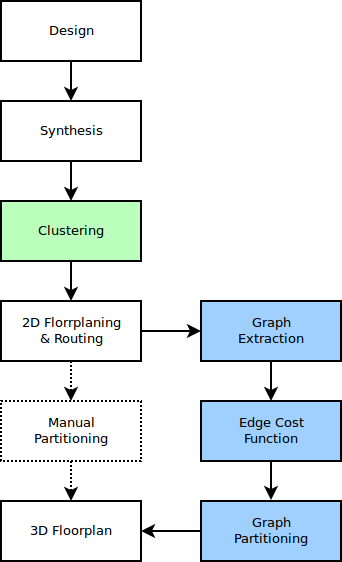
\includegraphics[height=0.85\textheight]{design-flow}
\end{frame}

\begin{frame}
  \frametitle{Objectives}
  \begin{itemize}
    \item Reduce interconnect length
    \item Reduce critical path length
    \item Reduce interconnect amount
  \end{itemize}
\end{frame}


\section{Definitions}
\begin{frame}
  \begin{definition}[Disjoint Partitions, \cite{Papa2007}]
    % Note: to span a definition on several pages, we can do something like:
    % \begi{frame}
    %   \begin{definition}
    %     foo
    %   \end{definition}
    % \end{frame}
    % addtocounter{definition}{-1}
    % \begin{frame}
    %   \begin{definition}[cont.]
    %     bar
    %   \end{definition}
    % \end{frame}

    \setstretch{1.5}% Change the line spacing for this group, requires setspace package.
    A k-tuple $P=(p_0, ..., p_{k-1})$  with each $p_i$ a set of vertices such that $\bigcup_{i=0}^{k-1} p_i = V$ with $\bigcap_{i=0}^{k-1} p_i = \emptyset$
    % Note: if you want the limits above the symbol: \bigcup\limits_{i=0}^{k-1}

  \end{definition}
\end{frame}

\begin{frame}
  \begin{definition}[k-Way Partitioning]\cite{Papa2007}
    A function of the form $\delta$
  \end{definition}
\end{frame}

\begin{frame}
  \begin{definition}[Hypergraph]\cite{Papa2007}
  \end{definition}
\end{frame}

\begin{frame}
  \begin{definition}[Cut]\cite{Papa2007}
  \end{definition}
\end{frame}

\begin{frame}
  \begin{definition}[Sum of External Degrees]
    As presented by \cite{Karypis1998:hmetis}:
    \[ \sum_{i=1}^k |E(P_i)| \]
  \end{definition}
\end{frame}

\begin{frame}
  \begin{definition}[Scaled Cost]\cite{Karypis1998:hmetis}
  \end{definition}
\end{frame}

\begin{frame}
  \begin{definition}[Absorption]\cite{Karypis1998:hmetis}
  \end{definition}
\end{frame}

\begin{frame}
  \begin{definition}[k-Way Hypergraph Partitioning Problem]\cite{Papa2007}
  \end{definition}
\end{frame}




%%%%%%%%%%%%%%%%%%%%%%%%%%%%%%%%%%%%%%%%%%%%%%
% 				BACKUP SLIDES
%%%%%%%%%%%%%%%%%%%%%%%%%%%%%%%%%%%%%%%%%%%%%%


% \begin{frame}[noframenumbering]
% \frametitle{Software GCM}
% 	\begin{figure}
% 	\input{ipsec-ping-benchmark-gcm}
% 	\caption{Software: asm kernel module mode GCM\newline{} Hardware: AES IP core mode CBC}
% 	\end{figure}
% \end{frame}




%%%%%%%%%%%%%%%%%%%%%%%%%%%%%%%%%%%%%%%%%%%%
\section*{References}
%%%%%%%%%%%%%%%%%%%%%%%%%%%%%%%%%%%%%%%%%%%%

% \nocite*{}
\bibliographystyle{plain}
\bibliography{../../thesis/bibliography}

\end{document}
